\documentclass[sigconf]{acmart}
\usepackage{cleveref}

\settopmatter{printacmref=false}
\setcopyright{none}
\renewcommand\footnotetextcopyrightpermission[1]{}
\pagestyle{plain}
\crefformat{section}{\S#2#1#3}
\begin{document}

%%
%% The "title" command has an optional parameter,
%% allowing the author to define a "short title" to be used in page headers.
\title{Suggesting Secure Implementation to Vulnerable Code Snippets on Stackoverflow.}


\maketitle
\section{Introduction}
\label{into}
In this project I want build a static analysis tool which will achieve the following. 
\begin{itemize}
\item  Analyze the code snippets from Stackoverflow for identifying out which part of the code is vulnerable and show warning signs to highlight that part of the code to the developer.
\item When developer clicks on the warning sign a secure implementation while be shown to the developers. In case of failure of building generating a secure implementation, the tool will show insightful/helpful messages explaing why this part of the code is flaged as insecure.  
\end{itemize}

% Give two pictures here.
\begin{figure}[ht]
  \centering
  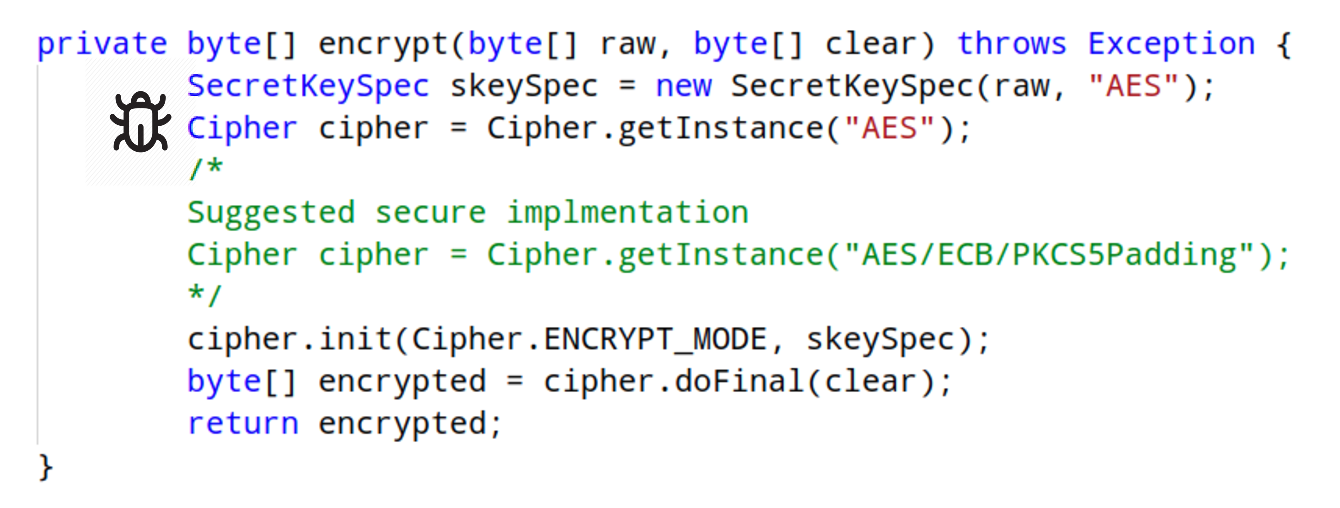
\includegraphics[width=\linewidth]{Figures/Selection_011.png.eps}
  \caption{A real code snippet taken from Stackoverflow. I want to build a tool which after analyzing the code snippet will highlight the part of the code that is insecure and suggest an alternative secure implementation as showed in the figure.}
  \label{fig:motivating-example}
\end{figure}

\section{Why the problem is interesting}
The problem is interesting for two reasons. 

\paragraph{Difficulty of writing crypto code securely.} Writing/implementing cypto code securely is a diffculut task for programmers. Any potential bug in crypto code can lead to serious vulnerablities open for attackers.
Even so unlike other code, crypto code can be insecure even if it works 
perfectly on traditional test-suite's input/output which is used only to prove the implementation correctness of the program.

\paragraph{Online platforms roles in spreading insecure code.} Online programming discussion platforms such as Stack Overflow have a rich source of ready to use code snippets for software developers. It is the defac-to place where developers go to find solutions of their problems and turn to the community for answers to their problems. 
Insecure code snippets found on Stackoverflow itself is not a serious problem. However,  
Fischer et al. has shown that developers have a tendency to directly copy paste code form Stack Overflow~\cite{fischer2017stack}. Therefore there are chances that any insecure code snippets posted on Stackoverflow can potentially find it way into production level code. To make matters worse, Meng et al.~\cite{meng2018secure} has showed that many accepted answers on Stackoverflow have seriously insecure code and often-times given by users having high reputation. This adds to the problem copy pasting vulnerable code from online platform and furthermore increases the chances of the insecure code snippet being trickled down to production level code. 
Unfortunately there is not state-of-the-art tool to analyzie if a code posted by developer on Stackoverflow is secure or not. In absense of such tool, Stackoverflow is potentially contributing as a major source of vulnerability in production level code.  

A static tool which can identify which part of the code snippet is insecure and suggest secure alternatives can help stopping the flow of insecure code from Stackoverflow to production level code.

\section{Proposed Methodology/Milestones}
As of now I am not really sure how to achieve the proposed goals described in \cref{into}. Especially how state-of-the-art synthesis techniques (e.g., program sketching) can be useful. However I am confortable analyzing insecurity of crypto code and therefore proposing the following methodology. 

My main idea is to convert the insecure and secure code snippets to AST and then apply synthesis to convert the insecure AST to secure AST \textit{somehow}. Again I am not sure about this synthesis part.  

\subsection{Data Collection}
I have collected code snippets from Stackoverflow which are publicly available in~\cite{fischer2017stack, meng2018secure}. They contain insecure code snippets of Java and Andrioid. Therefore, for now, I am planning to restrict myself to finding insecure code snippets in Java and Android only. 

\textcolor{blue}{
  I have done this. provide URL to the collected data.
}


\subsection{Identify Insecure Code Patterns}
I have manually analyzed the insecure code in ~\cite{fischer2017stack,meng2018secure}. I have already identified around 10 common insecure patterns which are most frequently occuring in them to an idea how secure code should look like.

\textcolor{blue}{
  show a table and code snippets in the appendix.
}
\subsection{Converting Code Snippets to AST}
Next, I am planning to convert the secure and insecure implementation to abstract syntax tree (AST) for comparing. This can be difficult since these code snippets are partially complete (i.e., missing classes, method implementations). However Fischer et al.~\cite{fischer2017stack} have done it by integrating partial program analysis (PPA) tool~\cite{dagenais2008enabling} with WALA\footnote{https://github.com/wala/WALA}. However how they have done it, is not explained by Fisher et al. in details. I have experiences using PPA~\cite{dagenais2008enabling}. However I am familiar with PPA, but have not used WALA yet. %I am thinking about emailing the authors if the proposed methodology is approved by you. 

\textcolor{blue}{
 here write that you are done with generating the AST
 The problem is annomyous class.
}

\subsection{Comparing AST of secure and insecure code}
This is the part I am mosting unsure of. I think synthesis will come handy here. 
I think the proper way should be finding the minimum changes we need to have to conver the AST built from insecure code to AST built from insecure code.  

If I can write first-order-logic for finding these minimum changes then that would be great. Because then I can use SMT solvers like Z3 to solve the constraints problem. 
So far I been unable to make progress in this direction and could not design the behavior constraints, structural constraints, and constraint solving part of the problem. I am also not sure how synthesis guided neural network can be useful or not. 

I have tried to go through the three papers on synthesis on the reading list of this course to get familiar with state-of-the-art techniques on program synthesis. I have some intuition. For example, repairing programs under uncertainty can be useful to synthesize code which needs to have IV/keys random with high entropy ~\cite{albarghouthi2017repairing}. Also I think Program sketching can be useful by placing holes in places where a cipher mode is used and writing assertion that any insecure ciphers can not used to fill up the hole.    

\section{Chanllenges}
I can think of the following challenges, I need to take care of while building the static tool.
\begin{itemize}
  \item The developed static tool needs to fast as if any developers post an insecure code it should not take much time to inform him/her that the code is not secure and where the problem is.
  \item It should not be too conservative (i.e, have low recall) and the same time high precision. Low recall will mean the static tool will always complain about the code snippet even if it is secure. Low precision means it will miss many of the insecure code snippets. We high precision and recall. 
\end{itemize}
\textcolor{blue}{
\section{Experimentation Evalutation}
%\section{Related work}
}
\bibliographystyle{ACM-Reference-Format}
  \bibliography{references}
  
\section{Appendix}

% evalutation plan on datasets.
\end{document}
\end{document}